\documentclass[preprint,12pt]{elsarticle}
\PassOptionsToPackage{hyphens}{url}
\usepackage{hyperref}
\usepackage{float}
\usepackage{natbib}
\journal{Atmospheric Environment}
\begin{document}
\begin{frontmatter}
	\title{
		Impact of unprecedented events on air pollution over a large industrial hub: Monterrey 2015-2022
	}
	\author[1]{Adriana Ipiña}
	\author[2]{Constanza Zúñiga-Villarreal}
	\author[3]{Gamaliel López-Padilla}
	\author[4]{Jair Rafael Carrillo Ávila}
	\author[5]{Michel Grutter}
	\affiliation[1]{
		organization={Instituto de Física Rosario (CONICET-UNR)},
		addressline={27 de Febrero 210 BIS},
		city={Rosario},
		postcode={2000},
		state={Santa Fe},
		country={Argentina},
	}
	\affiliation[2]{
		organization={Centro de Investigación Científica y de Educación Superior de Ensenada (CONAHCYT)},
		addressline={Carretera Ensenada - Tijuana 3918},
		city={Ensenada},
		postcode={22860},
		state={Baja California},
		country={México}
	}
	\affiliation[3]{
		organization={Centro de Investigación en Matemáticas A.C (CONAHCYT)},
		addressline={De Jalisco s/n, Valenciana},
		city={Guanajuato},
		postcode={36023},
		state={Guanajuato},
		country={México}
	}
	\affiliation[4]{
		organization={Agencia de la Calidad del Aire, Secretaría de Medio Ambiente de Nuevo León},
		addressline={Washington 2000 Ote},
		city={Monterrey},
		postcode={64010},
		state={Nuevo León},
		country={México}
	}
	\affiliation[5]{
		organization={Instituto de Ciencias de la Atmósfera y Cambio Climático, Universidad Nacional Autónoma de México},
		addressline={Investigación Científica s/n, CU},
		city={Ciudad de México},
		postcode={04510},
		state={Ciudad de México},
		country={México}
	}
	\vspace{-1em}
	\begin{abstract}
		The COVID-19 pandemic and subsequent restriction measures have been the subject of many studies about air quality. However, the impact of unprecedented meteorological and environmental events on air pollution in the same context has been very rarely investigated. This work presents an analysis of the pollutant concentrations along the passage of cold fronts, African dust, a hurricane, wildfires, and an atypical drought in the Monterrey Metropolitan Area (MMA) for the period 2015-2022. The average percentage changes with respect to baseline in PM\textsubscript{10}, PM\textsubscript{2.5} and SO\textsubscript{2} declined up to -14\%, with an increase of 20\% for O\textsubscript{3} and 10\% for NO\textsubscript{2} during the most strict COVID-19 lockdown. The smaller than expected changes were due to exceptional episodes as well as the uninterrupted activity from heavy transport vehicles, industries, and quarries. The PM\textsubscript{10} changes calculated with the random forest deweather method were aligned to the results from the anomalies formula. These findings are of particular interest in establishing methods for further understanding the influence factors and formulating a better air quality policy in large cities.%
	\end{abstract}
	%%Graphical abstract
	\begin{graphicalabstract}
		
\includegraphics[width=12cm]{COVID-19_lockdown.jpg}
	\end{graphicalabstract}
	%%Research highlights
	\begin{highlights}
		\item Unprecedented meteorological and environmental events changed air pollutants in an industrial hub during the COVID-19 lockdown.
		\item Air pollutant reductions were not as significant as have been reported elsewhere during pandemic restrictions.
		\item The deweather method and anomalies analyses showed that the change in PM\textsubscript{10} was not really much larger than the fluctuations obtained throughout the fitting baseline period.
		\item Aerosol from neighboring regions, countries, or even continents must also be considered to evaluate the local contributions and chart feasible goals for the reduction policies.
	\end{highlights}
	\begin{keyword}
		COVID-19 lockdown \sep meteorology  \sep environmental events \sep air pollutants \sep Monterrey
		%% keywords here, in the form: keyword \sep keyword
		%% PACS codes here, in the form: \PACS code \sep code
		%% MSC codes here, in the form: \MSC code \sep code
		%% or \MSC[2008] code \sep code (2000 is the default)
	\end{keyword}
\end{frontmatter}
\section*{Introduction}
The World Health Organization (WHO) recognizes that the disease burden associated with air pollution is similar to that of the biggest health threats in large metropolitan areas \citep{organization2021}. Moreover, assessing the changes in atmospheric photochemistry, meteorology, and pollution is essential for proposing effective policies on air quality. The COVID-19 pandemic provided an opportunity to study nitrogen dioxide (NO\textsubscript{2}), ozone (O\textsubscript{3}), particulate matter (PM), and sulfur dioxide (SO\textsubscript{2}) worldwide \citep{Kumari_2020}, as most countries implemented a mandatory lockdown to stop infection, unintentionally benefiting the environment \citep{Han_2022,Ravindra_2022}. The reduction in vehicle traffic and the closure of industrial operations led to a drop in atmospheric pollution \citep{Barr__2021,Sicard2020,Sharma_2020,Venter_2020}, especially in the major metropolises \citep{Saha_2022,Slezakova_2021}. In particular, NO\textsubscript{2} decreased along the full lockdown period in at least 63 cities around the world \citep{Sokhi2021}. In a similar way, the low PM\textsubscript{2.5} values reflected some degree of the partial and total activity shutdown in most cities \citep{Chauhan_2020,Saha_2022}, such as a decrease ranging from 5.93\% \citep{Bao2020} up to 46.5\% \citep{Xu_2020} in China and nearly 200\% in India \citep{Kotnala_2020}. These changes were generally much lower in some urban areas of Europe than in Asia \citep{Sicard2020,Fu_2020} and a slight increase in some US cities \citep{Zangari_2020,Archer_2020}. Since the COVID-19 disease was identified, China, India, and the USA lead the list of countries with publications about lockdown and air pollution, while Mexico is one of the most underexplored \citep{Aboagye}. Comparative studies with respect to prior periods have predominated, but few have examined the meteorological and environmental causes \citep{Hernández-Paniagua2021,Bontempi_2022,ZORAN}, and even less in the post-pandemic period \citep{Priya}. Although the pandemic restrictions provided great data to fill the knowledge gap about air pollutants, there are still unresolved questions about cities where the reduction was not significant. Monterrey Metropolitan Area (MMA) is an industrial development hub in northeastern Mexico, with more than 4000 foreign-capitalized companies accelerating urban growth \citep{20152018}. Furthermore, its proximity to the United States border maintains one of the principal commercial routes and an intense flow of heavy transportation \citep{cmm2019}. The Pan American Health Organization has recognized PM\textsubscript{10} in MMA as one of the highest in Latin America \citep{Riojas-Rodríguez2016}. Its particle composition includes black carbon (BC) \citep{Peralta_2019} sulfates, organic carbon (OC) \citep{Mancilla_2019} and Volatile Organic Compounds (VOCs), with a seasonal dependence on maximum photolysis and temperature \citep{Menchaca_Torre_2015}.
Carbonyl compounds increase in the morning and decrease in the afternoon \citep{j2012}, which are sensitive to the NO\textsubscript{x}--O\textsubscript{3} relationship \citep{Menchaca_Torre_2015a}. Likewise O\textsubscript{3} has a sensitive response to the changes in NO\textsubscript{x} and VOCs emissions, meteorology, and photochemistry \citep{Hern_ndez_Paniagua_2017}. Mobile sources are the main regional source of PM\textsubscript{2.5} and its precursors (NO\textsubscript{x}, VOCs, and NH\textsubscript{3}) \citep{Martínez-Cinco2016}. The state vehicle register enlists about 2 million, 700 thousand auto motors \citep{len}, that substantially contribute to metropolitan emissions. Recently, Tesla announced the construction of its largest plant in the world on the Monterrey outskirts \citep{tesla_2023}. This urban site is a key point for the investigation of economic growth, increasing emissions, and the energy transition. Consequently, the aim of this work is to analyze eight years (2015-2022) of air pollutant observations affected by unprecedented events in Monterrey, one of the largest cities in the Western Hemisphere \citep{Ni_2023}.
\section*{Materials and Methods}
\subsection*{Mobility and COVID-19 cases}
The \emph{Healthy Distance Program} was a countrywide strategy in Mexico based on social distancing measures and the closure of all non-essential activities \citep{covid-19a}. From the beginning of the pandemic, some local governments disagreed with the national recommendations, as was in the MMA \citep{state}. It implemented a mixture of measures from March 2020 to October 2021 (Table S1). Social media information was widely used as a measure of mobility during the lockdown. Figure S1 shows the COVID-19 cases \citep{covid19mex}, the mobility from a \emph{Python} library \citep{Graff_2022}, and the Unified Mobility Index (MIU) \citep{conacyt}.
\subsection*{Ground data}
The Integral Environmental Monitoring System (SIMA) records in MMA the criteria pollutants PM\textsubscript{2.5}, PM\textsubscript{10}, NO\textsubscript{2}, O\textsubscript{3}, SO\textsubscript{2}, and CO. Additionally, this network also collected meteorological data on humidity, temperature, global solar irradiance, precipitation, wind speed and direction. The available data for the period 2015--2022 were analyzed, except for the SE3 station that started operations in 2017. The CO measurements were not included because of a lack of calibration from 2016 to 2021. Figure \ref{596247} shows and lists the selected stations that comply with at least 75\% of the available monthly measurements per pollutant \citep{mtodos}.
\begin{figure}[H]
	\begin{center}
		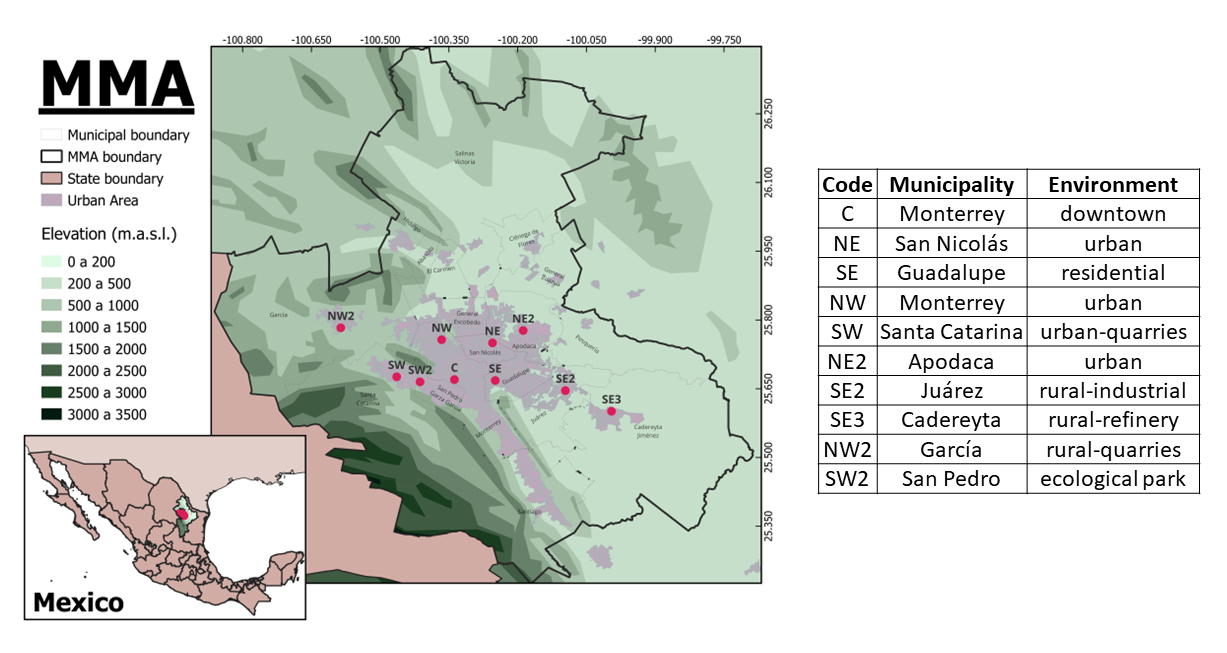
\includegraphics[width=0.70\textwidth]{figures/amm_tabla.png}
		\caption{SIMA stations (red dots) in the MMA.
				{\label{596247}}}
	\end{center}
\end{figure}
\subsubsection*{Deseasonalized air pollutants data and anomaly calculation}
A function derived from the linear term and truncated Fourier series was fitted with a frequency of \(K=2\), and its coefficients were obtained \citep{Hernández-Paniagua2021} for the baseline (January 2015 to December 2019). The air pollution anomalies \(A\left(t\right)\) were calculated as follows:
\begin{equation}
	A\left(t\right)=D\left(t\right)-\left[c_0+c_1t+ \sum_{k=1}^{K}\left(a_{k}\cos(2\pi tk)+b_{k}\sin(2\pi tk)\right)\right]
	\label{eq:anomalies}
\end{equation}
By subtracting the linear trend \((c_{0}+c_{1}t)\) and the Fourier fitting from the original air pollutant measurements \(D(t)\), the influence of seasonality and long-term trends were reduced. Considering meteorological conditions, the pollutant measurements in the presence of daily accumulated precipitation of 10 mm and wind speed values of 60 km/h were filtered.
\subsubsection*{Deweather model for PM\textsubscript{10} data}
Machine learning methods to determine changes in air quality have gained popularity over the past decades. Random Forest (RF) is a regression model that has been implemented to extract meteorological influences in air pollution \citep{Breiman_2001,Vu_2019,Cole_2020}. It involves applying a normalization technique to meteorology based on pollutant emissions  \citep{Stuart_2019,Zongbo_2021,Lv_2022}. The RF model was trained using measurements in the period 2015-2022, with resampling for each monitoring station. The algorithm inputs were the meteorological (relative humidity, temperature, pressure, direction, and velocity wind) and temporal (hour and Julian day) variables to predict the PM\textsubscript{10}. The RF process repeats hundreds to thousands of times until it obtains an average regression called Deweather. In this work, the Deweather model was a method to evaluate the monthly changes in PM\textsubscript{10} during lockdown, comparing the results with anomalies analysis.
\subsection*{Satellite data}
\subsubsection*{OMI}
The Total Ozone Column (TOC) \citep{dcio}, NO\textsubscript{2} Vertical Column Density (VCD) \citep{Lamsal_2020}, and maps of Aerosol Optical Depth at 500nm (AOD\textsubscript{500}) are provided by the Ozone Monitoring Instrument (OMI) on board the AURA-NASA satellite. The satellite overpass time is between 13:00 and 14:00 h CST for the coordinates of Monterrey downtown (25.40°N, 100.28°W, and 560m asl). The products used were OMTO3 (L2) v8.5 for TOC, OMNO2 (L2) v4.0 for VCD, and OMAERUVd (L3) v3 for AOD\textsubscript{500}. Gases information was utilized to determine concentration patterns. For maps of the incoming aerosols from Africa, the Giovanni platform was employed \citep{torres2008}.
\subsubsection*{VIIRS}
The satellite instrument of the Visible Infrared Imaging Radiometer Suite (VIIRS) \citep{Schroeder_2014} was used for tracking wildfires. Near Real-Time NOAA-20 (formally JPSS-1) VIIRS Active Fire detection product is derived collaboratively by NASA and National Oceanic and Atmospheric Administration (NOAA). VIIRS has local overpass times of approximately 01:30 -13:30 h with a spatial resolution of 375 m. The data product Fire Radiative Power \citep{earthdata} was processed to localize the active fire and estimate the number of hotspots related to wildfires on the mountain range (the Sierra Madre Oriental, henceforth SMO) nearby MMA.
\subsection*{HYSPLIT model}
The Hybrid-Single Particle Lagrangian Integrated Trajectory (HYSPLIT) model from NOAA - Air Resources Laboratory (ARL) \citep{Stein_2015} was executed on the Realtime Environmental Applications and Display System website to demonstrate dust transport. Data from reanalysis 2015–2022, stored on the HYSPLIT website, were applied for wind backward-trajectories simulations during African dust events.
\section*{Results and Discussion}
\subsection*{Unprecedented events}
The changes in pollutants during 2020-2022 were affected by COVID-19 measures as well as the passage of cold fronts, hurricane Hanna, African dust, wildfires and an atypical drought. The characterization of exceptional events allows us to determine the real air pollution reduction caused by anthropogenic causes.
\subsubsection*{Cold fronts}
The frontal systems crossing the northern hemisphere considerably affect the air quality along their transport pathways. As the cold front enters an urban area, the contaminated airmass from other regions can cause a sharp increase in PM\textsubscript{10} \citep{Kang_2019}. Figure S2 shows an extreme PM\textsubscript{10} value of 430$\mu$gm\textsuperscript{-3} after cold front arrival. At the end of 2019 and the beginning of 2020, the long persistence of the jet stream with westerly winds and widespread displacement toward Mexican territory increased the number of cold fronts \citep{yucatn}. This phenomenon caused low raw averages of PM\textsubscript{10}, PM\textsubscript{2.5}, and NO\textsubscript{2} (Figures S3 and S4). Mexico City also recorded this decline in January and February 2020, prior to the pandemic restrictions \citep{Vega_2021}. In mid-February 2021, an unprecedented winter storm crossed the United States, causing failures in the electricity system supply in Texas \citep{Doss_Gollin_2021,years} at the same time as a new closure (L2) in the MMA. The cold snap whipped as far as northeastern Mexico, decreasing temperatures by below 10°C along with particle matter (Figure S2). The air pollutants measured during the passage of the cold fronts were filtered for the analysis of anomalies.
\subsubsection*{African dust}
In June 2020, the strongest dust storm over the last two decades (dubbed \textit{Godzilla}) transported massive amounts of dust from Africa to the Americas \citep{Francis_2020}. The origin, transport, and deposition of dust associated with the PM\textsubscript{10} increase can be identified by comparing the AOD\textsubscript{500} and HYSPLIT model \citep{Yassin_2018}. Figure S5 illustrates the back trajectories from HYSPLIT about the main dust transportation routes from northwest Africa to the southeast part of the MMA. This was aligned with the AOD\textsubscript{500} records from the OMI satellite before and during the COVID-19 lockdown. Part of the satellite grid cells cover a mountain bend that acts as a barrier by accumulating particles \citep{Gonz_lez_Santiago_2011,Martinez_2012}. On the other hand, SIMA sensors registered the arrival of the dust storm modeled by HYSPLIT, exhibiting ridges on 16 July 2018 and 17 July 2020 (Figure S6). The dusty episodes during the June-July period have also been recorded in Puerto Rico (18.22°N, 66.52°W) \citep{Euphrasie_Clotilde_2020} and Houston (667 km northeast of Monterrey) coincident with the large-scale Saharan dust intrusion \citep{Bozlaker_2013} when the dry deposition peak over the eastern Gulf of Mexico \citep{Lenes_2012}. The dust is present year-round due to erosion of soil, unpaved roads, particle resuspension, and quarry activities. Notwithstanding, PM\textsubscript{10} values rise midyear when African dust arrives, exceeding the WHO air quality guidelines \citep{Prospero_2014}. As at other sites affected by Saharan dust outbreaks, these PM\textsubscript{10} measurements were removed \citep{Clemente_2022} before applying the anomaly formula.
\subsubsection*{Hurricane Hanna}
The number of systems that at least qualified as tropical or subtropical storms during the 2020 Atlantic hurricane season exceeded that of the previous record-holder (in 2005) \citep{stefano2021,Beven_2021}. The eye of Hurricane Hanna made landfall 500 km from Monterrey (Figure S7) with maximum sustained winds of 150 km/h and a minimum central pressure of 973 hPa \citep{conagua}. It was the last significant rainfall in the MMA, crossing the region at the end of July 2020 and dropping the daily PM\textsubscript{10} for four days (Figure S6). The maximum precipitation accumulated was 489 mm at SE3 station and 604 mm in the vicinity of NE station (25.73°N, 100.30°W). Table S2 shows the PM\textsubscript{10} averages in July for the years 2020 and 2019, with the effects of African dust and Hurricane Hanna and without both events, respectively. The mean percentage relative differences (RD) without measurements affected by these episodes was -0.4\%.
\subsubsection*{Wildfires}
\label{sec:wildfiles}
From March to May in the central region of Mexico, wildfires occur \citep{Bravo_2002}. Early in the spring of 2021, one of the most devastating forest fires in the last decade raged over the SMO. Wildfires destroyed almost 1000 hectares and forced the evacuation of roughly 400 people. The VIIRS and the Moderate Resolution Imaging Spectroradiometer (MODIS) on board the Terra-NASA satellite detected at least eight clusters of hotspots (active fires) visible in the forested region, with smoke flowing northeast \citep{web}. In 2022, a second historical record of wildfires was observed in the same area. Figure S8 depicts the daily number of hotspots between 2015-2022 detected by VIIRS and a map of active fires during the most critical period. For assessing impact, a weighted kernel function was applied to the PM\textsubscript{10} and the wind speed and direction measurements in a specific radius \citep{Henry2009,Petit_2017,Ji_2019}. Figure S9 shows the non-parametric regression for five stations from 13 to 18 March 2021. Wildfire increased the PM\textsubscript{10} values higher than 100$\mu$gm\textsuperscript{-3} with the dominant southeast wind. Smoke is partially responsible for the increase of monthly average PM\textsubscript{10} in March 2021 and 2022 (Figure S2). In Mexico City outskirts, it produces over 70\% of the principal fine particle mass \citep{Yokelson_2007} and several trace gases in northeast Mexico \citep{Mendoza_2005}. This PM\textsubscript{10} increase does not seem to have a relationship between O\textsubscript{3} monthly mean and the number of fire detections, as in other regions of Mexico \citep{Carbajal_2015}.
\subsubsection*{COVID-19 lockdown}
In general, the particle matter decline in the first two months of 2020 was due to the atypical number of cold fronts. Furthermore, the meteorological conditions led to high-ozone episodes and driven the dispersion and accumulation of pollutants during the lockdown period \citep{Tello_Leal_2021,Bera_2022,SULAYMON}. Despite 54.6\% of the population using their own vehicles as the main mode of transportation to work \citep{mxico} and more than 90\% of them having mobile internet connection \citep{inegi2021b}, PM and NO\textsubscript{2} did not show a proportional reduction to the MIU in 2020. This result was more in line with the transport of air masses and meteorological parameters than the vehicular flux reduction, similar to those of Rio de Janeiro \citep{Dantas_2020} and Ireland \citep{Spohn_2021}. The predominance of the decrease in pollutants without taking into account environmental and meteorological factors could be falsely attributed to the COVID-19 lockdown. The environmental episodes should be taken into account in lockstep \citep{Liu2020} and they can help other cities identify natural and anthropogenic influences.
\subsection*{Satellite NO\textsubscript{2} and O\textsubscript{3} changes}
The NO\textsubscript{2} VCD monthly averages derived from OMI data \citep{Lamsal_2020} were used to calculate the RD for Monterrey city (25.67°N and 100.30°W). The pixel size is 1°$\times$1° with grid boxes drawn around the city coordinates. Figure S10 shows the main NO\textsubscript{2} VCD reductions in April and October 2020, around -21\% and -19\%, respectively. The values are lower than half of those reported in other large cities \citep{Bauwens2020}. The lowest VCD was 31\% in August 2022, during a total opening of activities. A deseasonalized analysis from platform Air Quality/NASA based on satellite data for Monterrey indicated a slight change from March to June 2020 during L1. Indeed, two months before the COVID-19 lockdown, the values were lower than in that period \citep{quality}. In the case of the O\textsubscript{3} column from OMI, peaks appeared on December 2021 and November 2022, within variations lower than \(\pm\)10\% along the period, implicating the main changes were in the tropospheric ozone.

\subsection*{Air Pollutants long term and  anomalies}
The air pollutants were not spatially homogeneous in the MMA due to the orography, urban sprawl, and a wide variety of anthropogenic sources. At least three years before the pandemic outbreak, PM\textsubscript{10} PM\textsubscript{2.5} and NO\textsubscript{2} (at SE3) concentrations decreased. This fact could have caused the O\textsubscript{3} formation from increased UV radiation \citep{Ipi_a_2021}. Figure \ref{686668} shows the truncated Fourier series and the linear trends for the monthly means of criteria pollutants in the period 2015–2022. The highest values for PM\textsubscript{10}, PM\textsubscript{2.5} and NO\textsubscript{2} occur in wintertime when O\textsubscript{3} reaches the minimum values. By contrast, SO\textsubscript{2} had no clear annual pattern. The solar UV radiation is around two times higher in the summer than in the winter and it promotes the formation of ozone and the aging of organic aerosols. The PM\textsubscript{10} and PM\textsubscript{2.5} trends exhibited clear decreases on practically all stations, following prior findings \citep{Aguirre_L_pez_2022}, attributed to the government's corresponding policy related to the 2017 controls on quarries and industries. Higher levels of particle concentration were recorded in the western zone, consistent with the predominant wind direction from east to west \citep{Gonz_lez_Santiago_2011}. A drastic drop in SO\textsubscript{2} at SW station was caused by ceasing in a factory as the main source of emission. In the post-pandemic period (2021-2022), a regional extreme drought promoted severe pollution accumulation along with low wind speeds and the second opening stage (N2). Excluding ozone, an increase in the daily pollutant concentrations was noticed in the first half of 2022 at almost all stations. The downtown station (near the water supply service of Monterrey) recorded a significant increase in NO\textsubscript{2} linked to the passage of heavy trucks used as water pipes during the drought-related crisis.
\begin{figure}[H]
	\begin{center}
		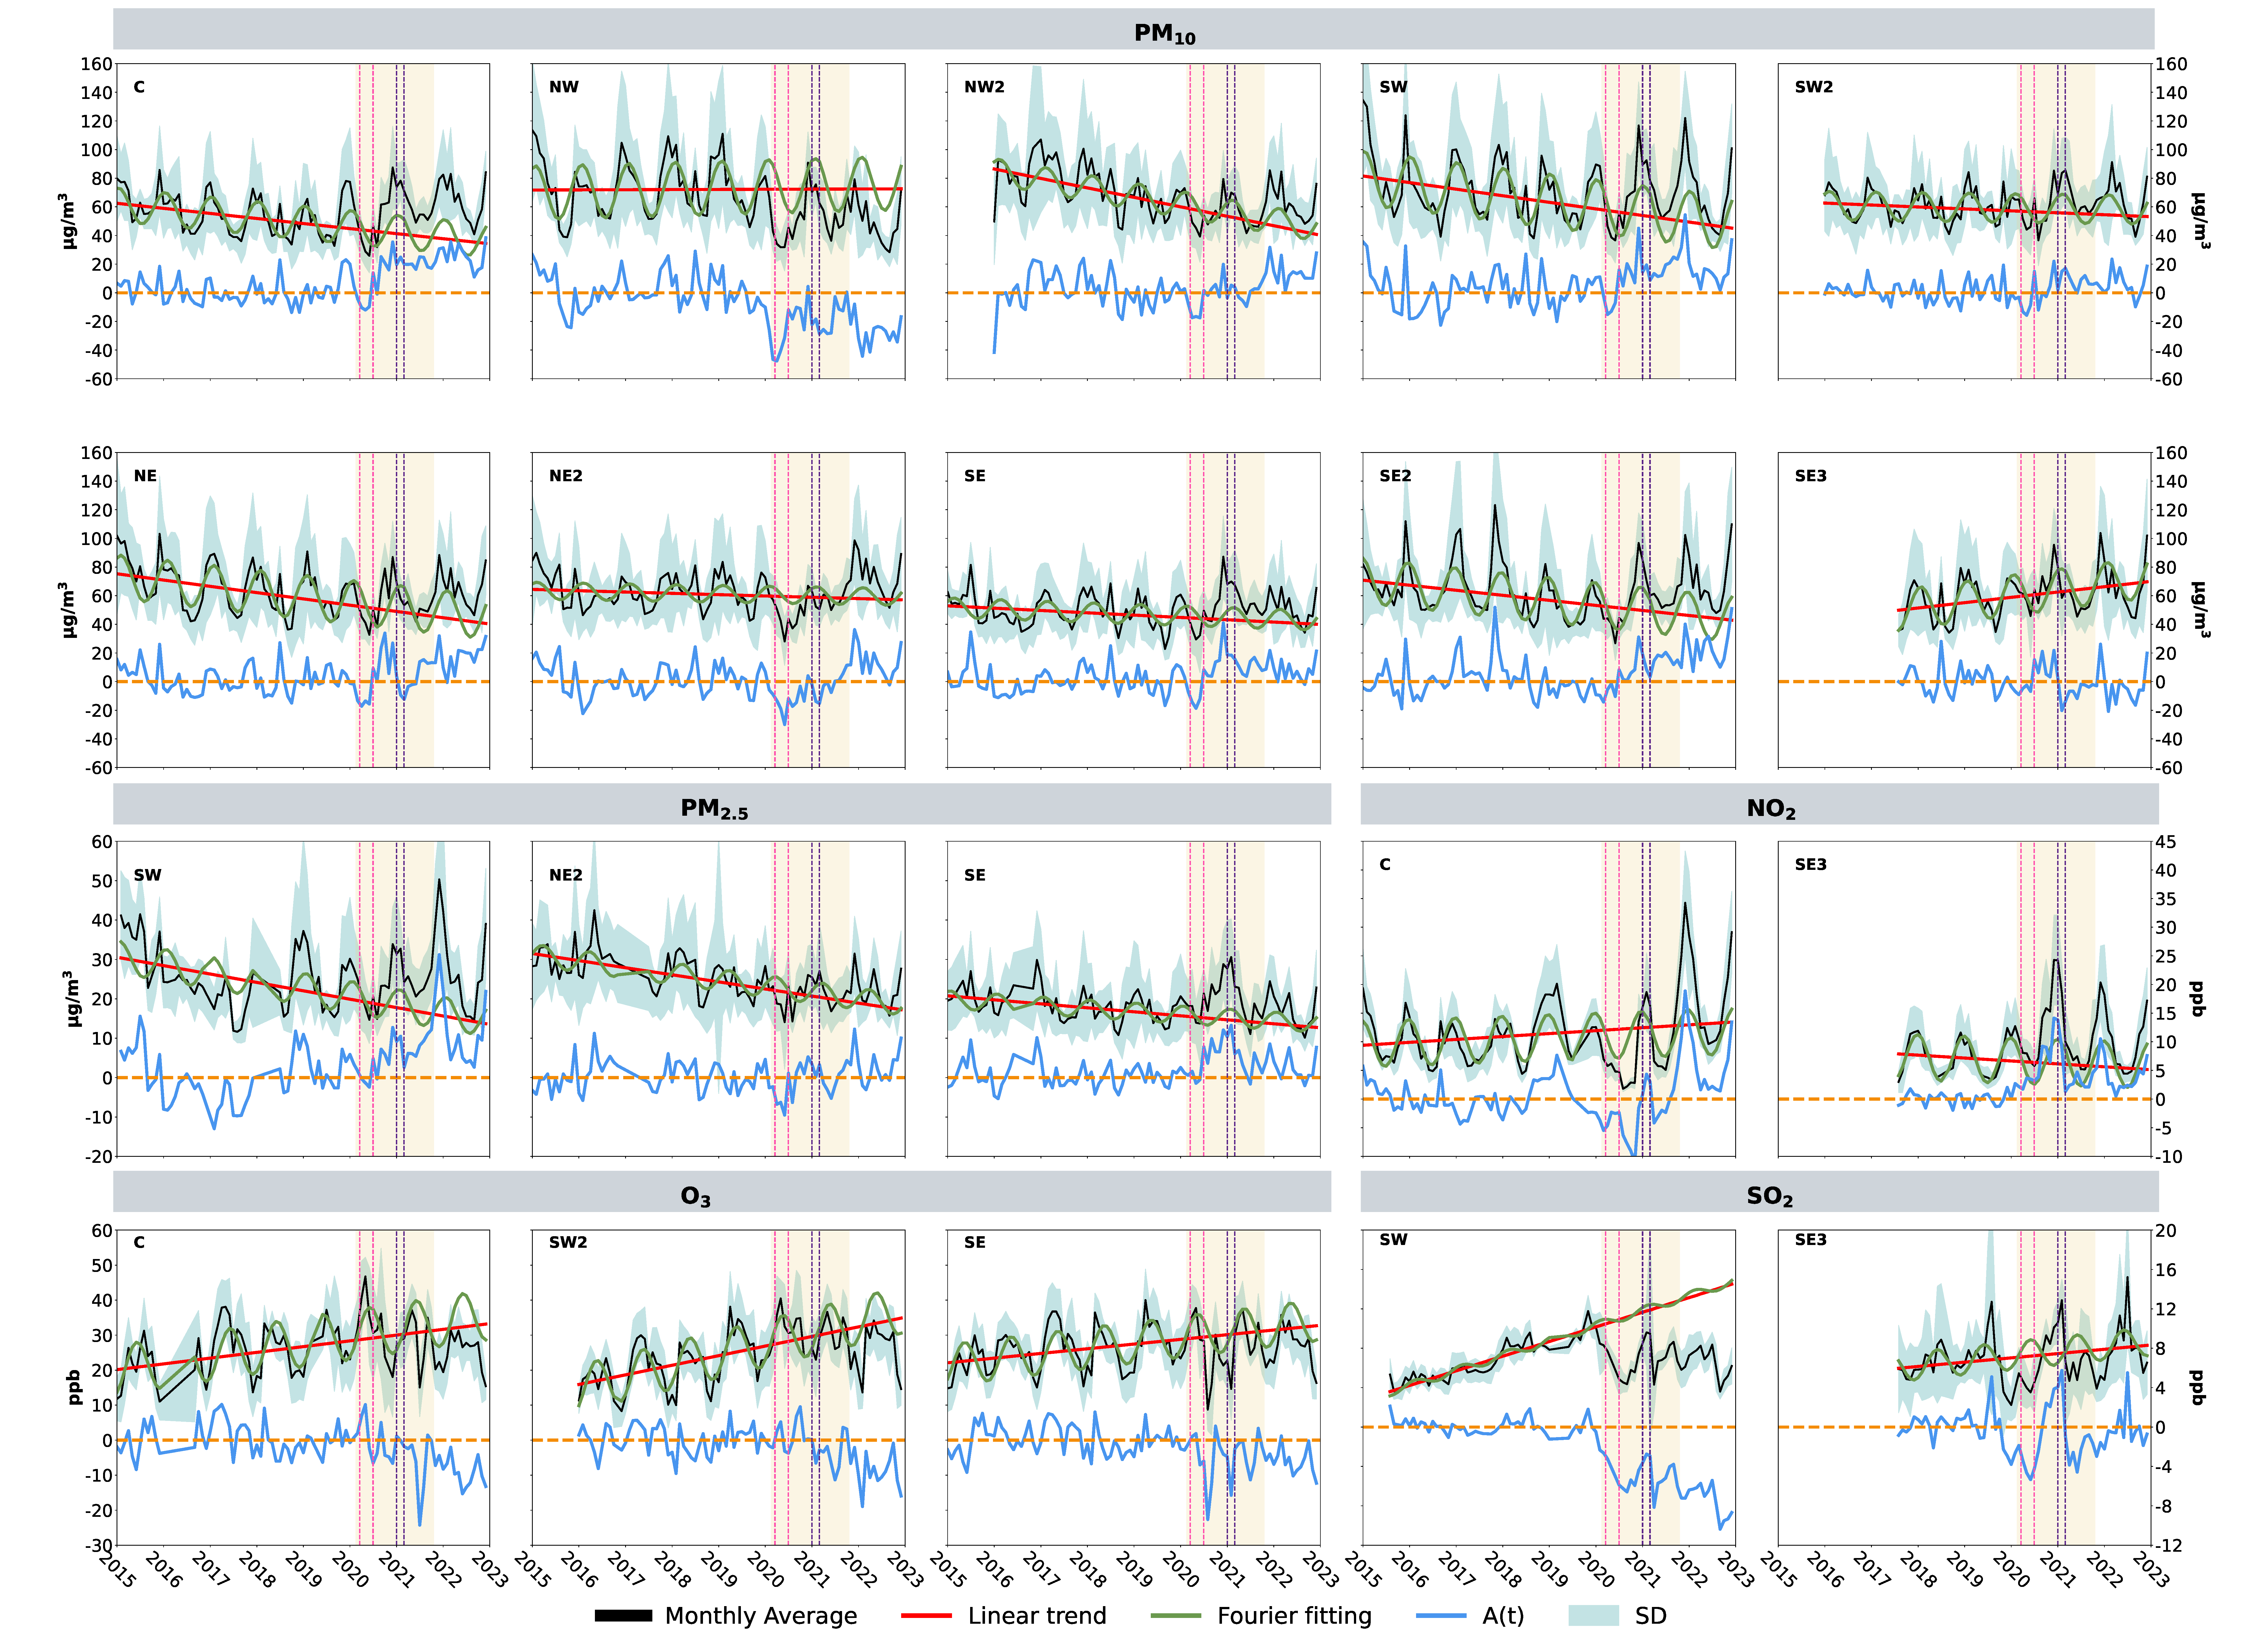
\includegraphics[width=1.00\textwidth]{figures/monthly_fourier.pdf}
		\caption{{Monthly averages of criteria pollutant concentrations recorded from 2015 to 2022 in the MMA, the linear trend, the Fourier fitting, and the anomaly A(t). The main lockdown were L1 (pink dotted line), L2 (violet dotted line), and the complete systematic phase (light yellow area).
						{\label{686668}}%
				}}
	\end{center}
\end{figure}
The trends decreased on average up to 2019 for PM\textsubscript{10} (-4 \%/yr), PM\textsubscript{2.5} (-7 \%/yr) and NO\textsubscript{2}(-1 \%/yr), while O\textsubscript{3} and SO\textsubscript{2} had an increase of approximately 8\%/yr and 14\%/yr, respectively (Table S3). The daily data set was filtered, considering meteorological and environmental factors. Subsequently, Equation 1 was applied to observe the net variation. The anomalies over the complete period exhibited values of \(A\left(t\right)<0\) not only in the lockdown context (Figure \ref{686668}). The baseline anomaly and overlapping years of 2020, 2021, and 2022 revealed the most noticeable changes were in PM\textsubscript{10} during L1, as shown in Figure \ref{313958}. The lowest anomaly was at NW, near the subway, encompassing high mobility and unpaved roads.
\begin{figure}[H]
	\begin{center}
		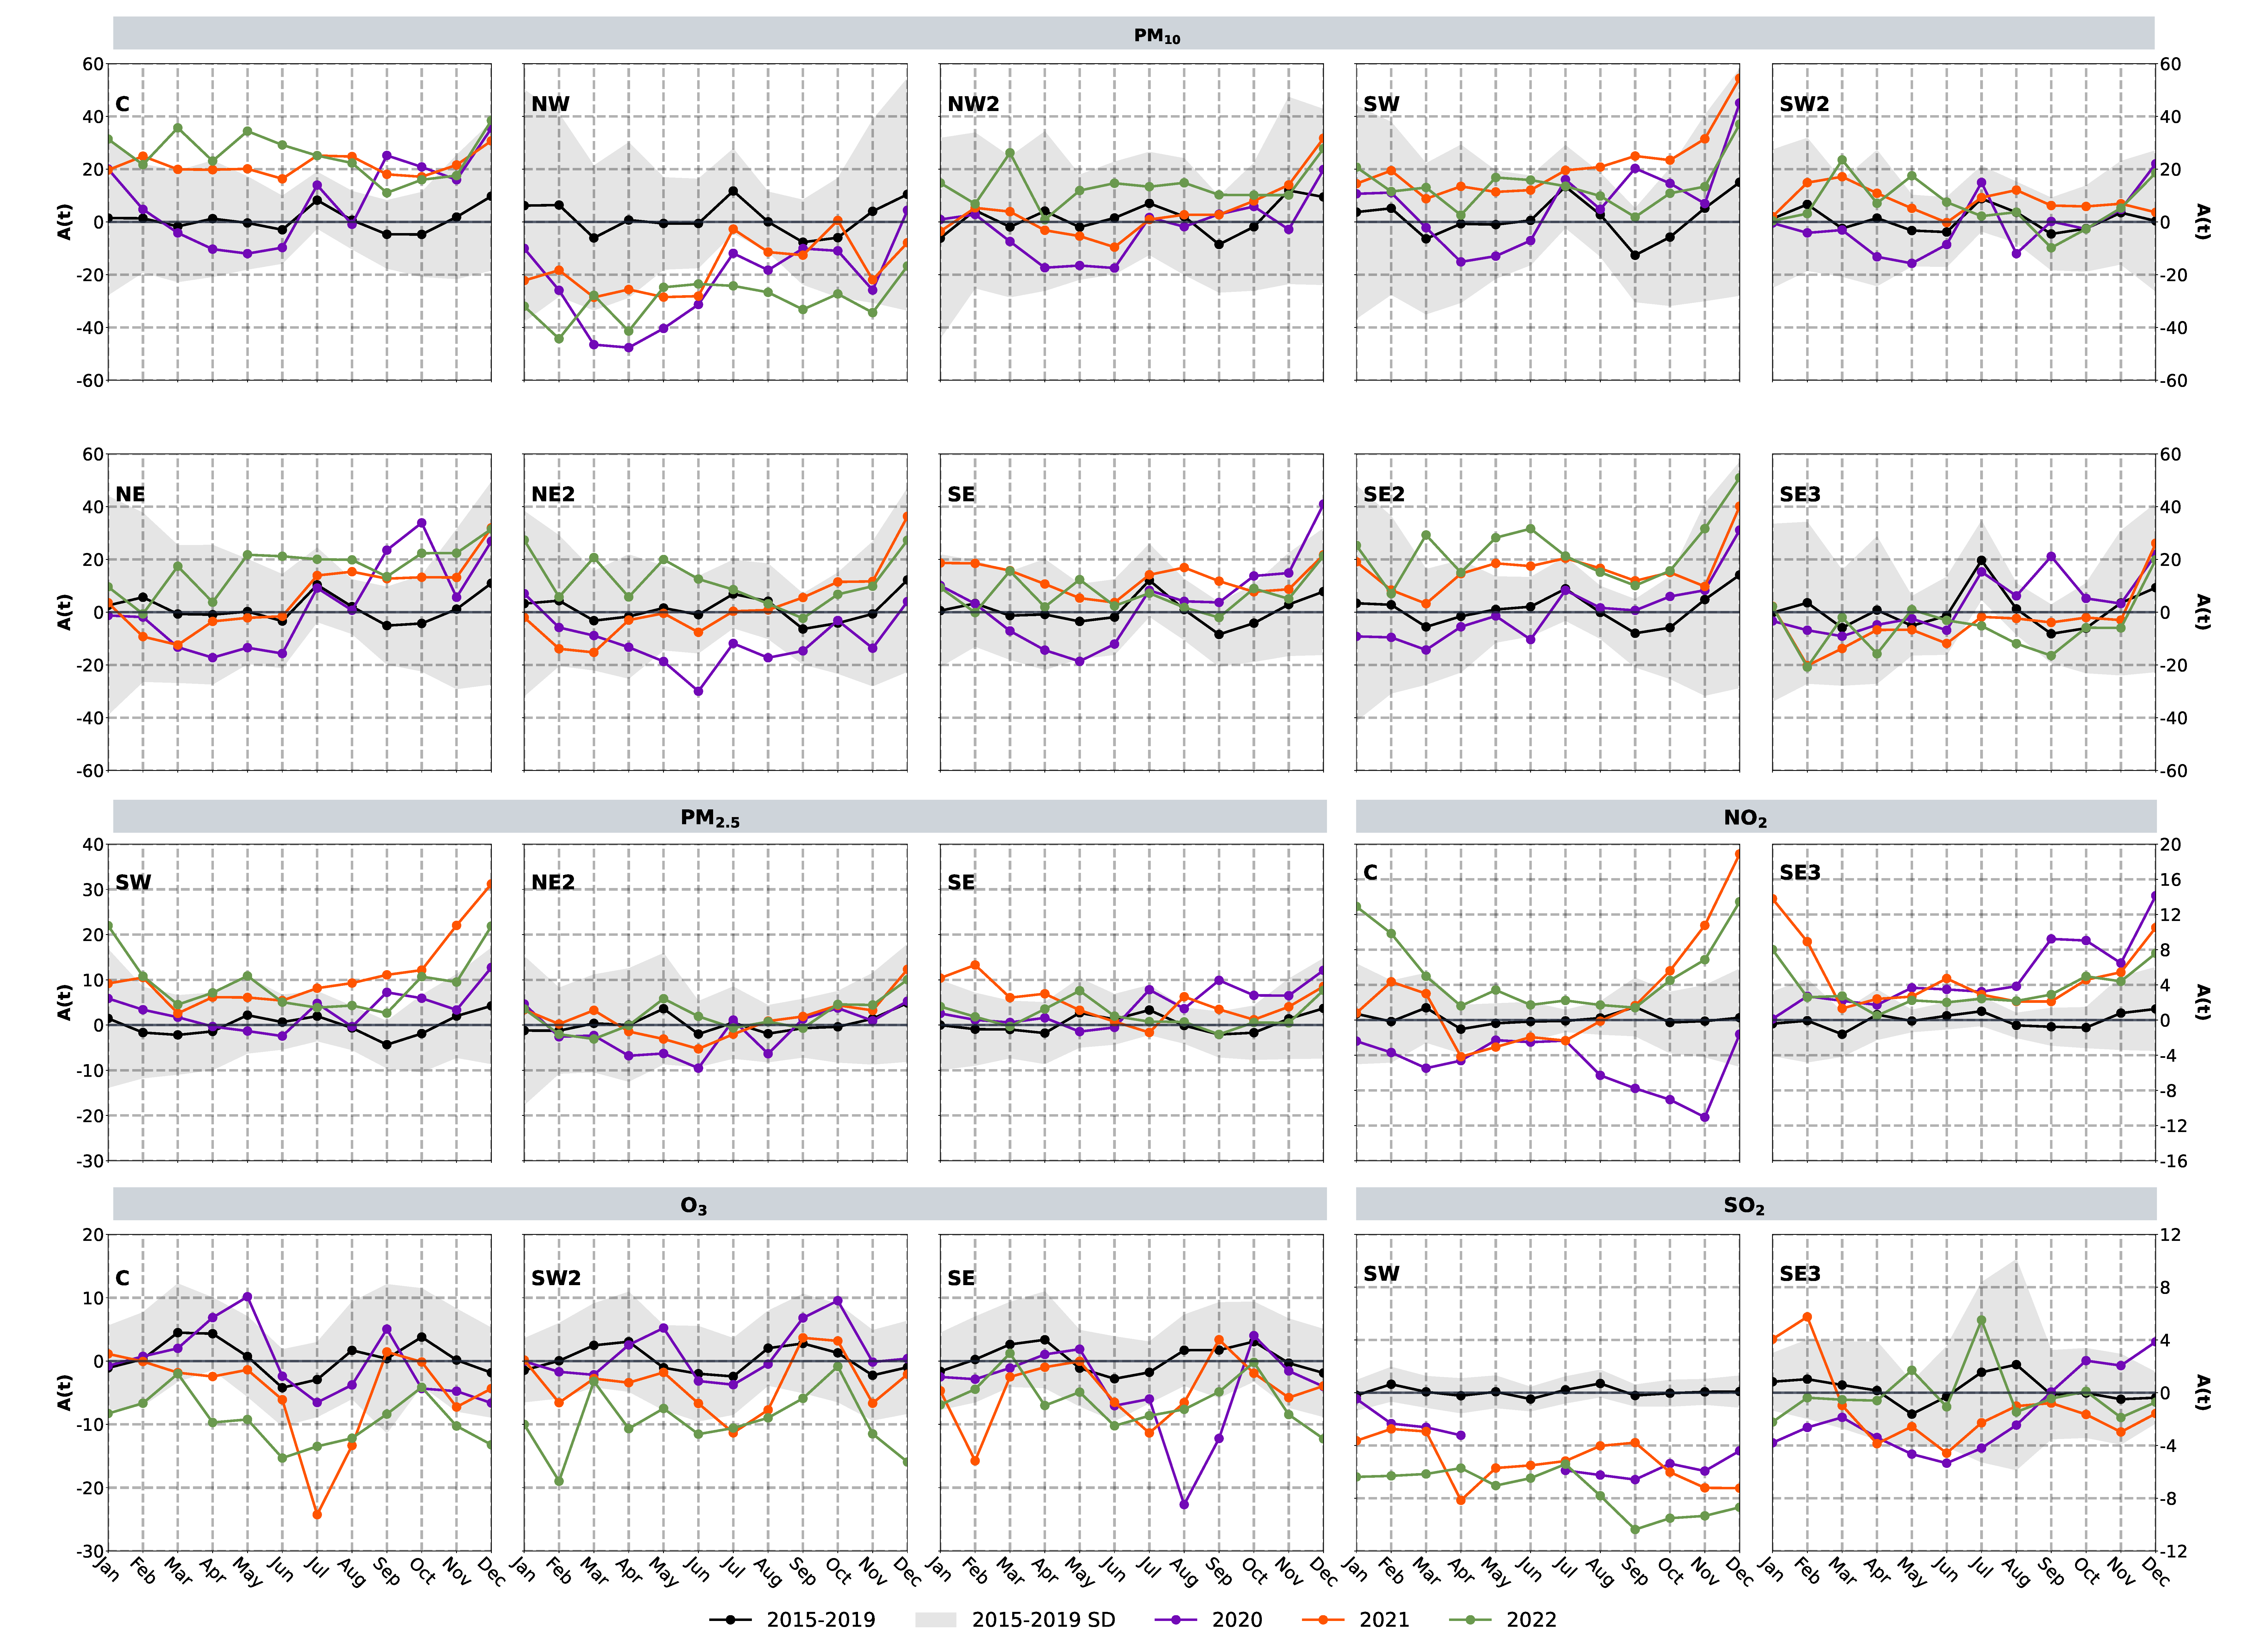
\includegraphics[width=0.98\textwidth]{figures/pollutant_anomalies.pdf}
		\caption{Monthly average anomalies of PM\textsubscript{10},
			PM\textsubscript{2.5}, NO\textsubscript{2}, O\textsubscript{3}, and
			SO\textsubscript{2} for the years 2020, 2021, and 2022, and the period
			2015-2019 with its standard deviation.
				{\label{313958}}}
	\end{center}
\end{figure}
The real average percentage changes during strict lockdown (L1) with respect to baseline in PM\textsubscript{10}, PM\textsubscript{2.5} and SO\textsubscript{2} declined up to -14\%, with an increase of 20\% for O\textsubscript{3} and 10\% for NO\textsubscript{2} (Table S4). The low reductions for PM\textsubscript{10}, PM\textsubscript{2.5} and NO\textsubscript{2} are consistent with the uninterrupted passage of heavy transport, which was considered an essential activity along with most industries. The ascending behavior at the end of 2021 and 2022 was present in the majority of pollutants, due to an exceptional drought period. The O\textsubscript{3} reached their maximum in the spring, followed by a prolonged slump until the early autumn coincident with the maximum UV solar intensity. In the cold dry season, the low photolysis rate might lead to a low conversion of SO\textsubscript{2} to sulfate ions and thus accumulate higher concentrations \citep{Gonz_lez_2018}. At least since September 2020, the decreasing of SO\textsubscript{2} could be inferred from the fact that several companies and industries in Sta. Catarina (SW) did not work during L1. The Cadereyta refinery near SE3 station had SO\textsubscript{2} and NO\textsubscript{2} levels below the baseline between 2021 and 2022 due to an improvement in the refinery emissions system in spite of uninterrupted activity and an intense drought.
\subsection*{Deweather model performance}
A special normalization of the meteorological effects on the PM\textsubscript{10} concentrations was carried out by means of the deweather-RF method. The results of ten metrics (Table S5) used to evaluate the deweather model performance aligned with the PM\textsubscript{10} values \citep{Lv_2022}. The non-linearity between predicted and observed values generated a mean Pearson correlation coefficient of 0.6, which is evidence of large differences due to extreme events. Figure S11 displays the behavior during the months involving relevant events.
\subsection*{PM\textsubscript{10} changes in extraordinary events}
The extraordinary events most significant were the COVID-19 restrictions (March 2020 to October 2021), storms (April 2020), hurricane Hanna, African dust (July 2020), cold fronts (February 2021), and wildfires (March 2021). Figure \ref{fig:average_change_deweather_fourier} shows the monthly mean PM\textsubscript{10} changes with respect to the baseline using raw data, the deweather model and the anomaly formula in the absence of environmental and meteorological episodes. An apparent reduction occurred by subtracting only the absolute values, except in the month of wildfires. Instead, the net changes calculated by Eq.\ref{eq:anomalies} were minor compared to the raw data, with differences more than twice and even opposite. Despite the fact that the deweathering method did not account environmental phenomena such as wildfires and African dust, the results were more similar to anomalies with filtered data. It demonstrates the relevance of considering these factors because they can inverse the changes in air pollution.
\begin{figure}[ht!]
	\centering
	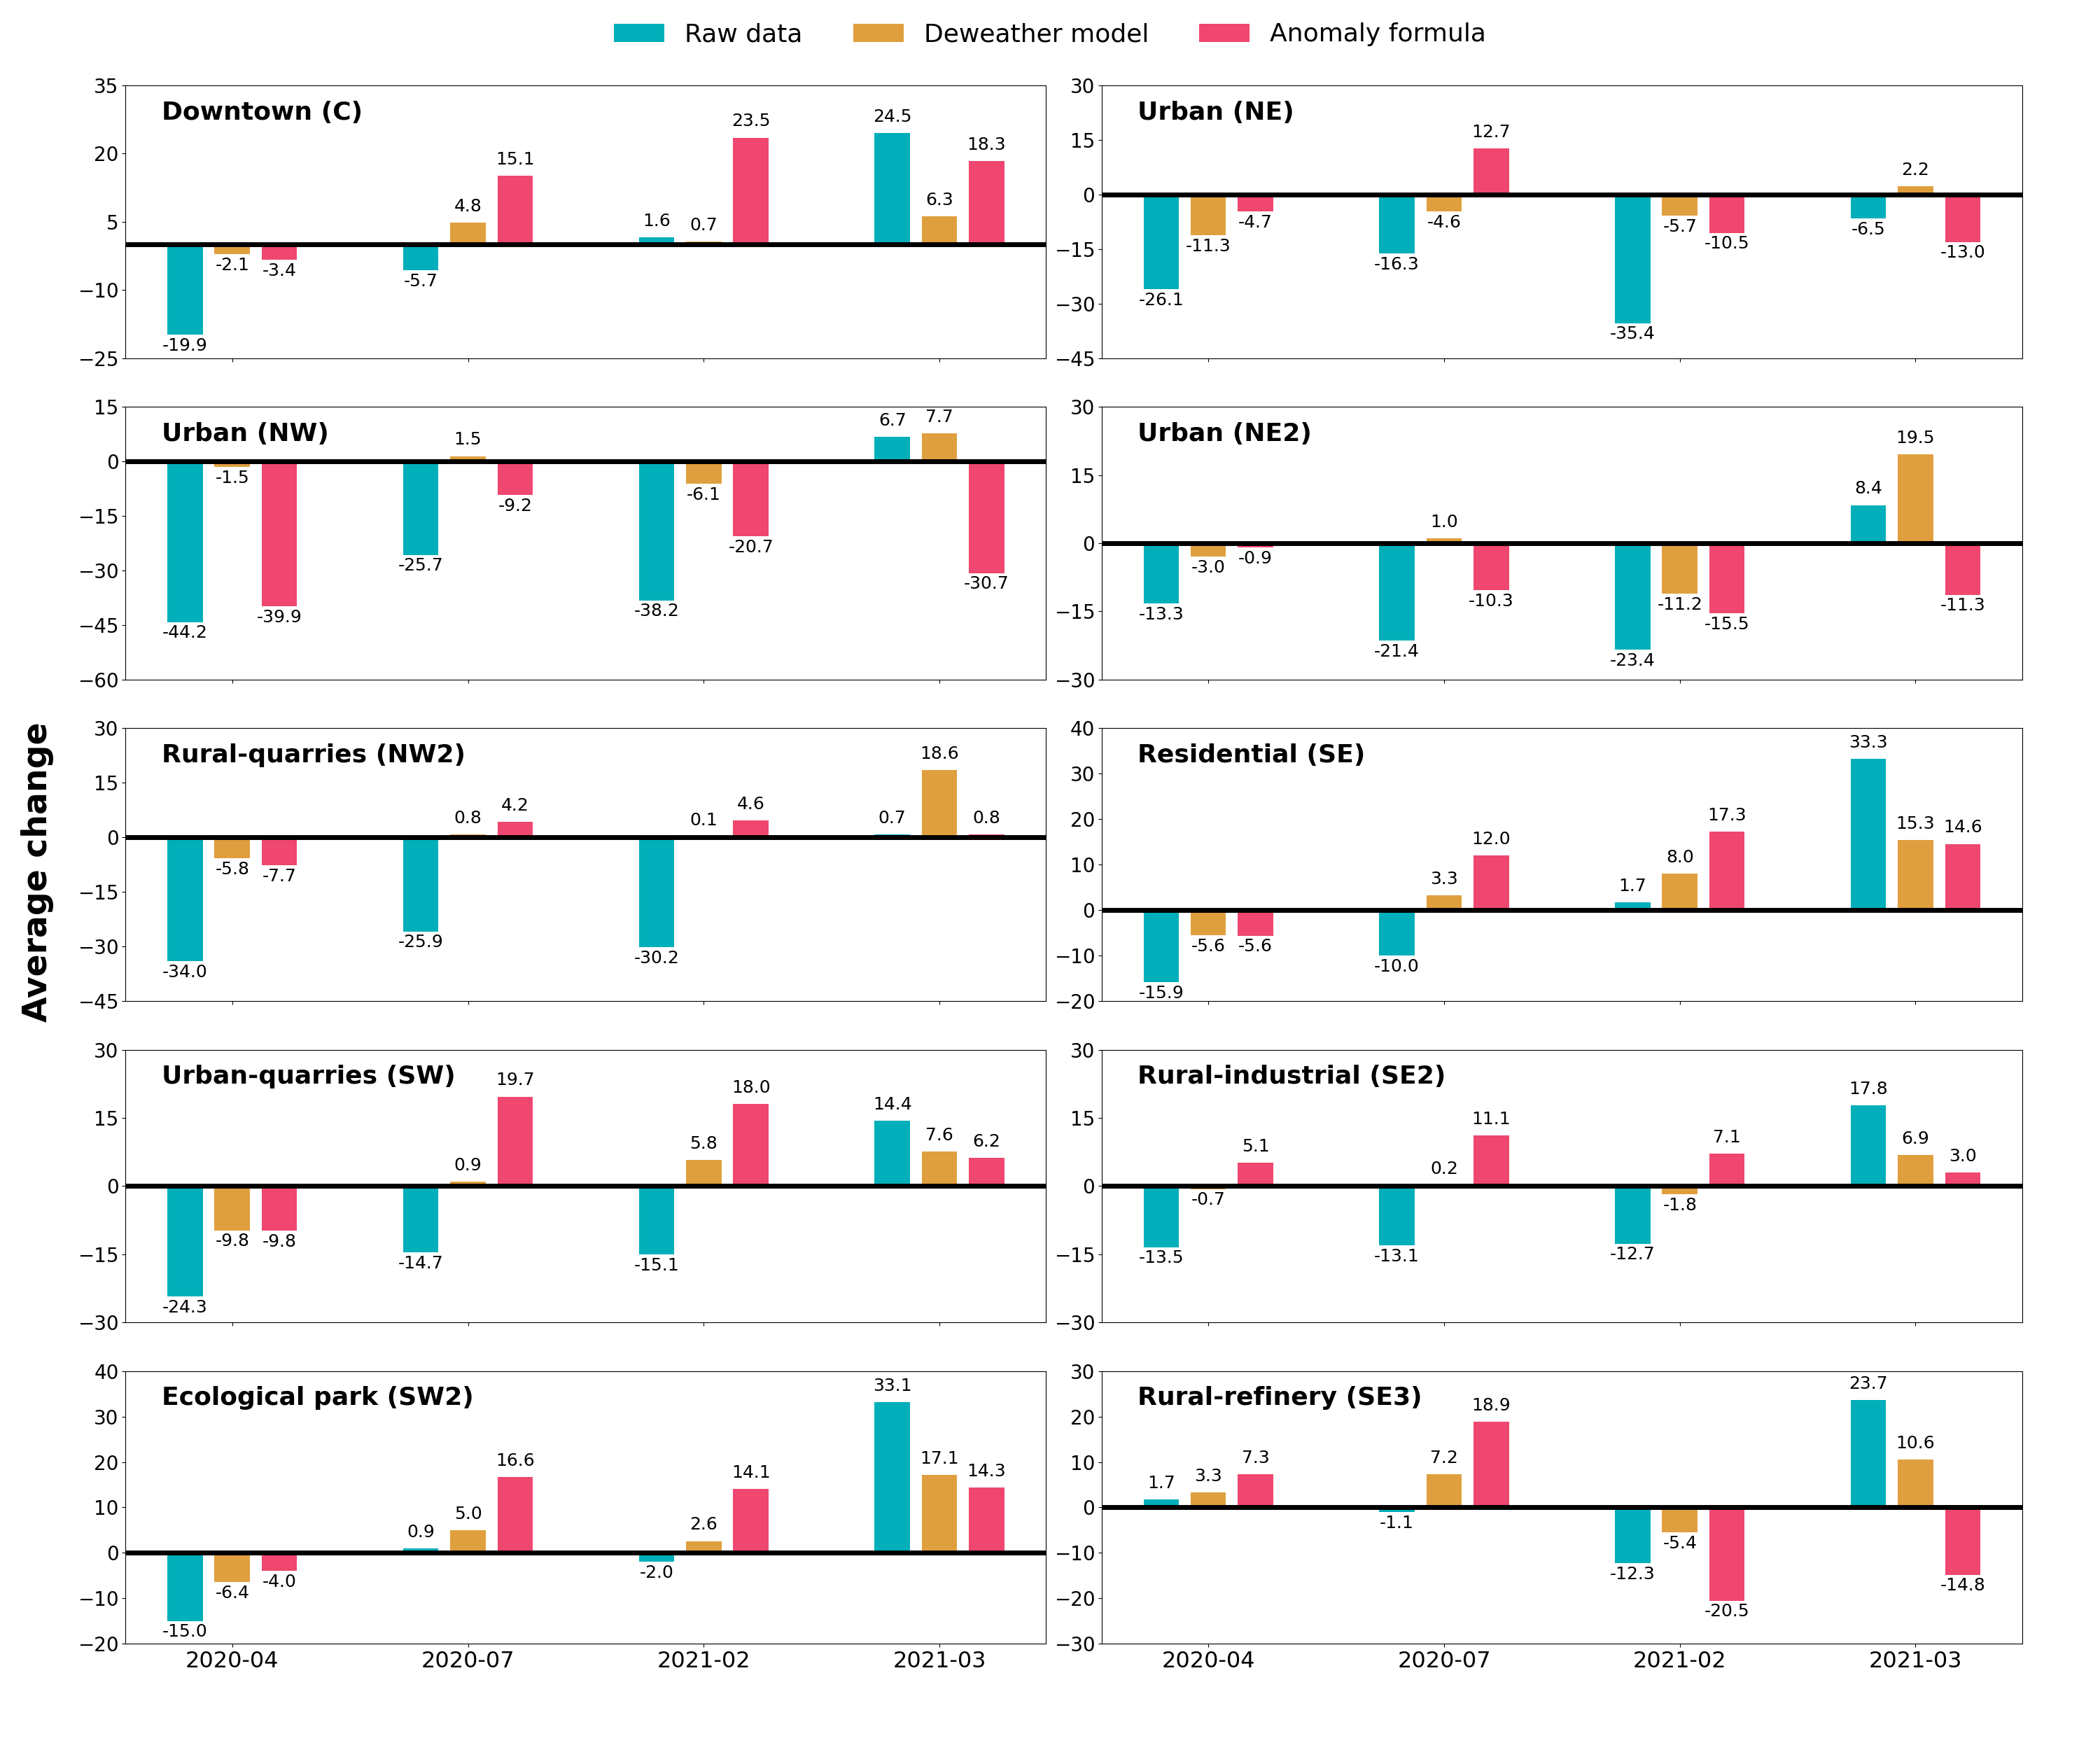
\includegraphics[width=\linewidth]{figures/average_change_deweather_fourier.png}
	\caption{Monthly mean changes of PM\textsubscript{10} with respect to baseline using raw data, the deweather model, and the anomaly formula. The last two take into account the passage of storms (April 2020), hurricane Hanna and African dust (July 2020), cold fronts (February 2021), and wildfires (March 2021).
	}
	\label{fig:average_change_deweather_fourier}
\end{figure}
\section*{Conclusion}
This study seeks to provide a broader picture of changes in atmospheric pollution, identifying the impacts of exceptional environmental and meteorological episodes and even controls prior to the COVID-19 health crisis. Unprecedented events affected the air quality from the beginning of 2020 to 2022 in a region with an industrial heritage and continuous growth. The influence of storms, cold fronts, wildfires, African dust, hurricane Hanna, an atypical drought and the COVID-19 lockdown on pollutant concentrations in the MMA was analyzed. The MIU from social media reflected the opening-closure stages of the non-essential activities in the COVID-19 measures rather than the changes in air pollutants.  Considering meteorological events by means of two methods, it revealed that the pollutant concentration changes during L1 were not really much larger than the fluctuations obtained throughout the baseline period. Nevertheless, it is crucial to account for extraordinary environmental episodes such as wildfires and dust arrivals in models to accurately understand and simulate the long-term trends of pollutants. Consequently, there was no 'background atmosphere' over the MMA in the pandemic restrictions, as has been reported elsewhere, since the heavy transport, the larger factories and companies were considered essential activities, and they worked as usual. Thus, it is important to continue to probe methods for decoupling influence factors and formulate a better air quality policy in large cities over a complex topography.
\section*{Acknowledgments}
The authors would like to thank the Nuevo León State government's Sistema Integral de Monitoreo Ambiental for providing the measurements. AI thanks Armandina Valdez of the Air Quality Agency for the management support, Mario Graff for the advisory about the IM method, Lok Lamsal (NO\textsubscript{2}) and Michael Yan (O\textsubscript{3}) for satellite data. CZV and GLP thank CONAHCYT for their fellowships.
\bibliographystyle{elsarticle-num-names}
\bibliography{bibliography/references.bib}
\end{document}
